\documentclass{llncs}
\usepackage{makeidx}
\usepackage[utf8]{inputenc}
%\usepackage{graphics}
%\usepackage[pdftex]{graphicx}
\usepackage{listings}
\usepackage{float}
\usepackage{graphicx}  

\begin{document}

\title{Waypoint navigation for an airplane UAV using MAVlink in JdeRobot framework}
\author{José Antonio Fernández\inst{1} \and Jose María Cañas Plaza\inst{2}}
\institute{Universidad Rey Juan Carlos}
\titlerunning{Article Abv}
\maketitle

\begin{abstract}
In order to make accesible to \texttt{JdeRobot} the command sets of \texttt{MAVLink} a driver is needed. The \texttt{APM Server driver} ``translates'' the \texttt{JdeRobot} interfaces objects in \texttt{MAVLink's} commands an viceversa, giving access to sensors and actuators of the robot. With the typical \texttt{JdeRobot} architecture applications can run in different machines (not necessarily aboard) and can be writen in different programming languages. 
In our case this driver run in a \texttt{Raspberry Pi3} with \texttt{raspbian OS} aboard the plane
\end{abstract}

\section{Introduction}

In order to address the problem of the waypoint navigation in JdeRobot a new driver, application and interface was developed  

\section{UAV support in JdeRobot}

JdeRobot is a software robotical enviroment developed in Universidad
Rey Juan Carlos's robotics laboratory. It is composed by utilities, drivers, interfaces and appications.
JdeRobot in the current version (at this time 5.5) present several drivers and applications in order to support UAVs.
One of these drivers is \texttt{ardrone server} who bring complete access to Parrot's AR-Drone sensors and actuators. Other of these drivers allow to simulate this same drone in Gazebo preventing devices damages produced by not tested software and develop more complex software tested in dificults simulated enviroments.
\texttt{UAV Viewer} is the most important JdeRobot application to teleoperating drones, allow to the operator robot's speed control and display all the attitude and onboard camera information.
JdeRobot is composed too with ZeroC ICE interfaces. This interfaces describe the objects sended between drivers-applications-utilities. Four of this current version was used in this project: \texttt{Camera}, \texttt{Extra}, \texttt{Pose3D} and \texttt{NavData}. \texttt{Pose3D} and \texttt{NavData} are used to retieve sensors measures, the first contains attitude information and position and \texttt{NavData} contains more sensor measures like linear velocities or battery level. In order to understand better these interfaces the following lines present the \texttt{Pose3D} and \texttt{NavData} implementation.

\begin{verbatim}
Pose3DData
  {
	float x;  //latitude
	float y;  //longitude
	float z;  //altitude
	float h;  //not used now
	float q0; //quaternion component 1
	float q1; //quaternion component 2
	float q2; //quaternion component 3
	float q3; //quaternion component 4
  };
  
\end{verbatim}

\begin{verbatim}
class NavdataData 
{
 int vehicle; //0-> ArDrone1, 1-> ArDrone2
 int state; // landed, flying,...
 float batteryPercent; //The remaing charge of baterry %
		
 //Magnetometer Ardron2.0
 int magX;
 int magY;
 int magZ;
		
 int pressure; //Barometer Ardron2.0
 int temp;     //Temperature sensor Ardron2.0
 float windSpeed; //Estimated wind speed Ardron2.0		
		
 float windAngle;
 float windCompAngle;
 
 float rotX; //rotation about the X axis
 float rotY; //rotation about the Y axis		
 float rotZ; //rotation about the Z axis
 
 int altd; //Estimated altitude (mm) 

 //linear velocities (mm/sec)
 float vx;
 float vy;
 float vz;
		
 //linear accelerations (unit: g) ¿Ardron2.0?
 float ax;
 float ay;
 float az;

 //Tags in Vision Detectoion
 //Should be unsigned
 int tagsCount;
 arrayInt tagsType;
 arrayInt tagsXc;
 arrayInt tagsYc;
 arrayInt tagsWidth;
 arrayInt tagsHeight;
 arrayFloat tagsOrientation;
 arrayFloat tagsDistance;

 float tm; //time stamp
};
\end{verbatim}


\section{MAVlink protocol}

\texttt{MAVLink}, MAVLink Micro Air Vehicle Communication Protocol is a drone's open source comunication protocol.  \texttt{MAVLink} was first released early 2009 by Lorenz Meier under LGPL license and pretends to be the standard in drone comunications and several drones like all the 3DRobotics company develoved drones.
Below it's described one of them in order to know this protocol.

\begin{verbatim}
<message id="33" name="GLOBAL_POSITION_INT">
	<description>The filtered global position 
	(e.g. fused GPS and accelerometers). The 
	position is in GPS-frame (right-handed, Z-up).
	It is designed as scaled integer message 
	since the resolution of float is not 
	sufficient.	</description>
<field type="uint32_t" name="time_boot_ms" units="ms">
	Timestamp (milliseconds since system boot)</field>
<field type="int32_t" name="lat" units="degE7">Latitude, 
	expressed as degrees * 1E7</field>
<field type="int32_t" name="lon" units="degE7">Longitude, 
	expressed as degrees * 1E7</field>
<field type="int32_t" name="alt" units="mm">Altitude in 
	meters, expressed as * 1000 (millimeters)</field>
<field type="int32_t" name="relative_alt" units="mm">
	Altitude above ground in meters, expressed as 
	* 1000 (millimeters)</field>
<field type="int16_t" name="vx" units="cm/s">Ground X 
	Speed (Latitude, positive north), expressed as 
	m/s * 100</field>
<field type="int16_t" name="vy" units="cm/s">Ground Y 
	Speed (Longitude, positive east), expressed as 
	m/s * 100</field>
<field type="int16_t" name="vz" units="cm/s">Ground Z 
	Speed (Altitude, positive down), expressed 
	as m/s * 100</field>
<field type="uint16_t" name="hdg" units="cdeg">Vehicle 
	heading (yaw angle) in degrees * 100, 0.0..359.99 
	degrees. If unknown, set to: UINT16_MAX</field>
</message>
\end{verbatim}

One example of this incoming message is:
\begin{verbatim}
GLOBAL_POSITION_INT {time_boot_ms : 480614, lat : -
353632612, lon : 1491652301, alt : 584110, 
relative_alt : -179, vx : 0, vy : 0, vz : 0, hdg : 
35608}
\end{verbatim}

To ensure message integrity a CRC is calculated to every message into the last two bytes. Another function of the CRC field is to ensure the sender and receiver both agree in the message that is being transferred. It is computed using an ITU X.25/SAE AS-4 hash of the bytes in the packet, excluding the Start-of-Frame indicator (so 6+n+1 bytes are evaluated, the extra +1 is the seed value).

To help us to build and understand these messages the driver uses \texttt{pymavlink}.


\section{APM driver in JdeRobot}

In order to make accesible to \texttt{JdeRobot} the command sets of \texttt{MAVLink} a driver is needed. The \texttt{APM Server driver} ``translates'' the \texttt{JdeRobot} interfaces objects in \texttt{MAVLink's} commands an viceversa, giving access to sensors and actuators of the robot. With the typical \texttt{JdeRobot} architecture applications can run in different machines (not necessarily aboard) and can be writen in different programming languages. 
In our case this driver run in a \texttt{Raspberry Pi3} with \texttt{raspbian OS} aboard the plane.

\subsection{Design}
\label{sec:design}

The driver has to fullfil the following features:

\begin{itemize}
\item Have to be able to connect to a physical devices like APM 2.8 but as well as to a simutator.
\item Have to access to sensors measures of the aereal robot and interpreting the data and serve its as ICE interfaces objects.
\item Have to be able to recieve incoming commands as ICE interfaces objects and send its to the devices as \texttt{MAVLink's} commands.
\end{itemize}

\begin{figure}[h]
  \centering
  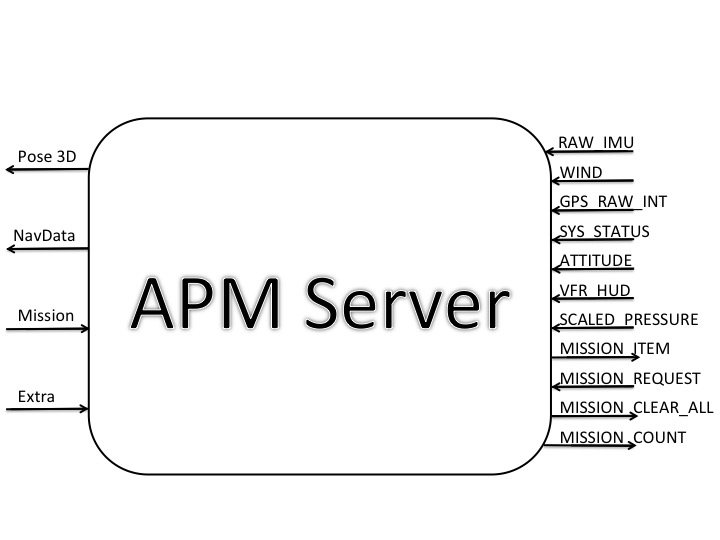
\includegraphics[scale=0.5]{img/diseno.jpg}
  \caption{\texttt{APM Server} inputs and outputs}
  \label{fig:diseno_apms_caja_negra}
\end{figure}

In order to adress it, a Python in \texttt{JdeRobot} component has been developed who implements all of above features called \texttt{APM Server}. 
\texttt{APM Server} is organized in three logical layers.
\begin{itemize}
\item Comunication's layer with APM's devices. ensures the establishment and maintenance the comunication with the APM device through \texttt{MAVLink's} commands.
\item Bussiness Layer. In this layer the driver convert form \texttt{MAVLink's} commands to ICE interfaces objects and viceversa.
\item \texttt{JdeRobot comunication's layer} This layer create all the ICE servers needed and handle incoming and outgoing ICE interfaces objects.
\end{itemize}


\subsection{APM data reading}
\label{subsec:apm_data_reading}

The driver can read \texttt{MAVLink's} commands from a physical device as \texttt{Pixhawk} or from a simulated drone in SITL simulator. The way to connect to each devices is choosed in the object instantation moment, we can choose to input the device's serial conection URI or the URL to the SITL simulator like udp:127.0.0.1:14550 in the connection sentence. Once the connection is established several \texttt{MAVLink's} messages start to be stored in the connection object buffer.
The driver handle eleven commands of the full set of \texttt{MAVLink's} commands (see Figure 1) to allow the \texttt{JdeRobot} integration. and in order to retrieve the APM sensors measures through this \texttt{MAVLink's} commands in the APM communication layer, a thread is ejecuting a message handler all the time.
In this handler, the asociated method, searchs for seven types of messages (like GLOBAL\_POSITION\_INT) which contains the needed data to fill the two ICE interfaces that the server serves: \texttt{Pose3D} y \texttt{NavData}.
The driver has four threads more, one for each of these ICE's interfaces servers, which binds four objects, so if a certain values are seted in these objects automatly are seted in the remotes binded objects this is the way to send information in ICE and the JdeRobot's applications comunication's layer.


Note in order to improve the connection speed and consumption is posible to set up the messages's set as you need.


\subsection{Sending missions to APM}
\label{sec:mission_apm}

This is the most important part of the driver. The driver recieve two ICE interfaces from comunication's layer with APM's devices, one developed in this project called \texttt{mission} with the waypoints to follow and the \texttt{Extra} interface with the take off and land maneuvers. This new ICE interface is composed from a list of \texttt{Pose3D} that contains the waypoints position that the plane has to reach. Its definition is showed in the following lines.

\begin{verbatim}
class Pose3DData  //we consumes Pose3DData
  {
	float x;  //latitude
	float y;  //longitude
	float z;  //altitude
	float h;  //not used now
	float q0; //quaternion component 1
	float q1; //quaternion component 2
	float q2; //quaternion component 3
	float q3; //quaternion component 4
  };

  ["python:seq:list"] sequence<Pose3DData> PoseSequence; // list of Pose3DData
  /**
  * Mission data information, Pose3DData sequence. 
  */
  class MissionData
  {
    PoseSequence mission;
  };

  /** 
   * Interface to the Mission.
   */
  interface Mission
  {
    idempotent MissionData getMissionData();
    int setMissionData(MissionData data);
  };
\end{verbatim}

Once a mission is received through these interfaces objects, \texttt{APM Server} build the \texttt{MAVLink's} commands needed to sent it to the APM. To perform it, a new thread with a listener was developed in order to know if there is a incominf mission.
Once this listener detects an incoming mission, call to \texttt{setMission(self, mission)} who build the \texttt{MAVLink's} commands and sent it as the Figure 2 diagram shows.
The \texttt{setMission(self, mission)} method is responsible to read througth the list of waypoints present in \texttt{Pose3D}-like creating all the \texttt{MAVLink's} commands needed to reproduce it sequence of waypoints in mission-like. If \texttt{takeOffDecision} and \texttt{landDecision} of \texttt{Extra} object are seted (\texttt{Extra} extra is one of the ICE interface objects binded) to True add the \texttt{MAVLink's} commands of take off and land at first and last of the list of commans which is sended to the APM.
At first we clear all existing missions in device and send to it the mission's items number we pretend to send. Then the device will request to the driver each one of these item sorted, one at time until the last is sended. 

\begin{figure}[h]
  \centering
  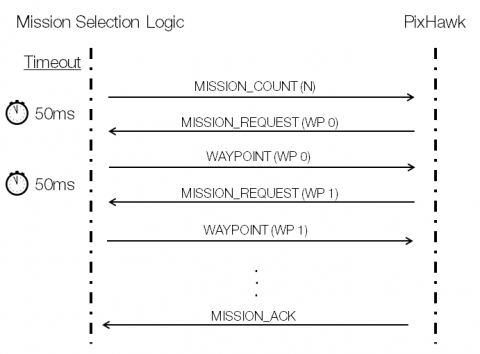
\includegraphics[scale=0.70]{img/waypoint-protocol-sendlist.png}
  \caption{\texttt{MAVLink's} missions sending protocol}
  \label{fig:misiones_mavlink}
\end{figure}


\section{UAV Commander application}

\texttt{UAV Commander} is a JdeRobot application writen in python in order to offer to a human operator build and sent missions to an autonomous \texttt{MAVLink} plane.

\subsection{Design}
\label{design}

The application has to fulfill the following features:
\begin{itemize}
\item The application have to display all the sensors measures data.
\item Have to get a friendly end user interface what allow to build missions and follow its compliance.
\item Have to be able to send the builded mission to the drone.
\end{itemize}

\begin{figure}
\centering{
   \label{f:diseno_uavc_caja_negra}
    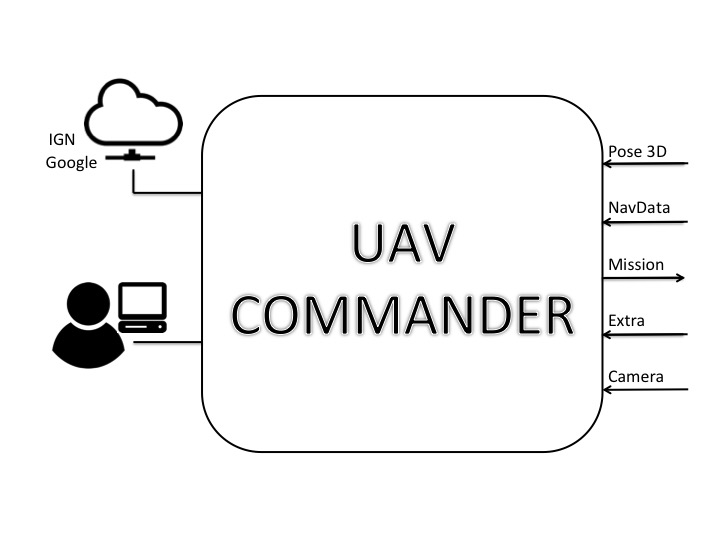
\includegraphics[width=1\textwidth]{img/diseno2_uavc.jpg}}
    \caption{\texttt{UAV Commander} input and outputs}

\end{figure}



The application is composed by 3 blocks: maps's block, missions's block and sensors's block. The maps's block is who adquire the maps and converts coordinates between diferent references systems. The missions's block allow to a human operator to build and sent missions and the sensors's block displays all de received sensors's measures data, onboad camera included.

\texttt{UAV Commander} connects to \texttt{APM Server} throught the  \texttt{Pose3D}, \texttt{NavData}, \texttt{Extra} and \texttt{mission} ICE interfaces, and can receive images and video throught \texttt{camera} from sources like JdeRobot's \texttt{cameraserver} driver.

\begin{figure}[h]
  \centering
  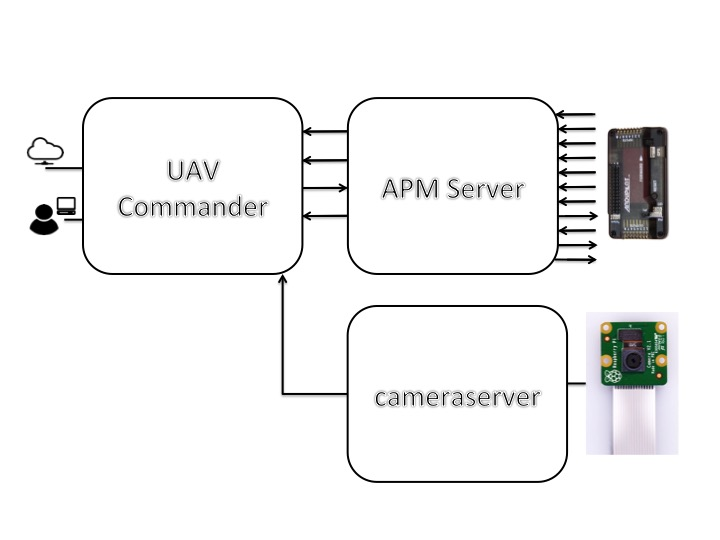
\includegraphics[scale=0.5]{img/arquitectura.jpg}
  \caption{\texttt{UAV Commander} and \texttt{APM Server} connection schema}
  \label{fig:uavc_ppal}
\end{figure}

\subsection{Maps's block}
\label{maps_block}

In this block the application download from Web Service Maps (WMS) a georeferenced map (the current version supports ``Instituto Geográfico Nacional de España'' (IGN) and Google as sources). For retrive these maps a few data is needed as: current possition (tatitude and longitude), the specific area to retrieve or bounding box, the desired image's resolution (in pixels) and the \textit{datum} or the Earth desired projection.
The WMS response is a map of the bounding box delimited zone. The pixels distribution of an image start in zero to the max widht of the image (from left to right) and start in zero to the max height of the image (from up to down). So with this image and de input data its possible to infer the coordinates of a specific pixel in the image.
In the current version of \texttt{UAV Commander} we agreed to despreciate the Earth curvature as long as we suppose the drone's missions local (less than 2 kilometers of radius) and these calculations are really simple.

\subsection{Missions's block}
\label{missions_block}

In this block the map is displayed and becomes interactive in order to help operator to build missions. If the maps is clicked in whatever position the application detects it, draw the waypoint mark in the map, infer the gographical possition and add that to the waypoints table. And if a previous waypoint was created, the application will draw the path from it to the new waypoint. Also is possible to make maneuvers like take off and land using the ``Take off/land'' button, pushing it and in a point of the map a take off is requested and the same in land maneuver.
In order to display the mission's tracking a complex layer system was developed, \texttt{UAV Commander} uses three layouts,  each one enriches the others. The first layer is the original downloaded image, is needed in case of a reset request, the second one comes frim the original too but is updated with a shadow in all the reached positions with the plane. And over this last layer the waypoints and the plane tracking and heading (the plane position are represented whit a triangle who rotates in order to reveal the heading of it) is drawed. This design allows resetting the map, clear the waypoints and not lost the shadows and tracking the plane with these all information.
In order to update all these information in the Graphical User Interface (GUI) a new thread was developed.
In order to don't loose the plane into its tracking an auto zomm feature has been developed. So in each update iteration the position over the image is chacked and if this position is closer to the borded (we decided less than one tenth of the widht or height) a new map will be downloaded with the double bounding box that the original.
All these features are available from \texttt{UAV Commander} main window.

\begin{figure}
  \centering
  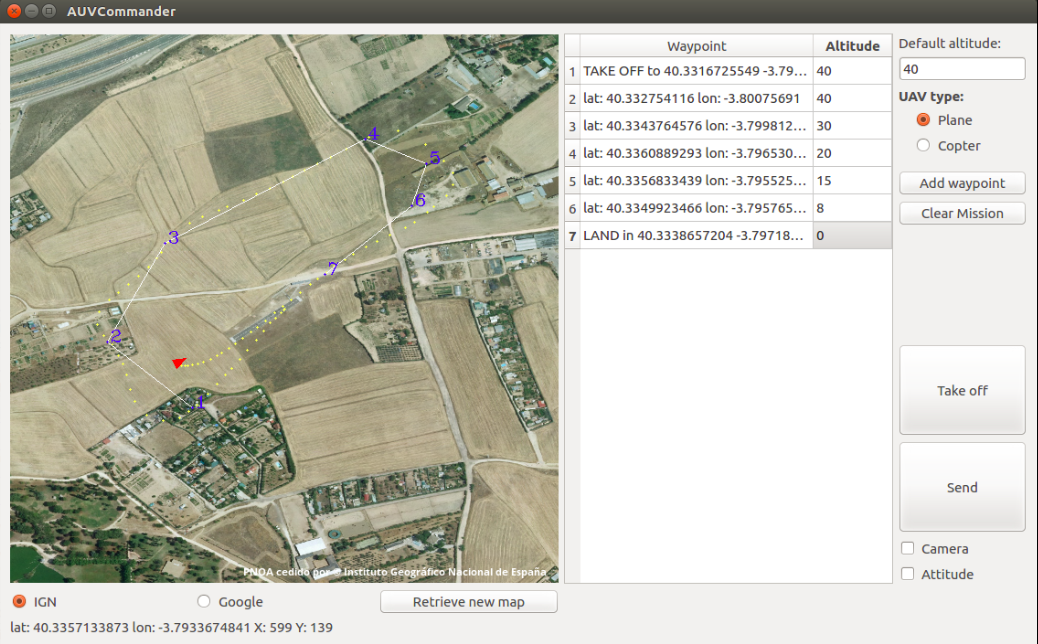
\includegraphics[scale=0.33]{img/uavc_mission.png}
  \caption{\texttt{UAV Commander} main window}
  \label{fig:uavc_ppal}
\end{figure}

\subsection{Sensors's block}
\label{sensors_block}

Here the sensors's measures data are displayed in way to be more understandables to the operator, in order to enrich the missions's tracking. This data is recovered from the APM Server in ICE interfaces objects, exactly Pose3D and NavData but has Camera ICE interface too so can receive images and video by this way, with JdeRobot's cameraserver driver for example. All these information are interpreted and displayed in the sensor's and camera's windows.
In the Figure 6 

\begin{figure}
\centering{
   \label{f:actitud_uavc}
    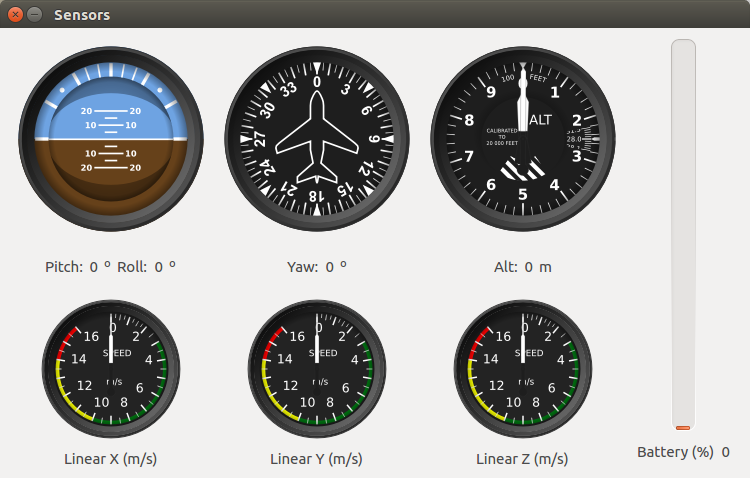
\includegraphics[width=1\textwidth]{img/actitud.png}}
    \caption{\texttt{UAV Commander} attitude and battery load}
  
\end{figure}

\section{Conclusions}

In order to give mission support to JdeRobot a new driver called \texttt{APM Server}, a new application called \texttt{UAV Commander} and a new JdeRobot interface was developed.

In order to tests the driver and the aplication several experiment was designed and as we need to test both develotments in a simulated enviroment an in a real prototype. All the experiments are uploaded to YouTube and are available in the following URL \url{https://www.youtube.com/user/cbyte18}. The day to day work was written in the following mediawiki \url{http://jderobot.org/Jafernandez} and all the developed software is in GitHub in \url{https://github.com/RoboticsURJC-students/2014-pfc-JoseAntonio-Fernandez}

\end{document}
